
\phantomsection
\section*{Глава 2. Проектирование веб-приложения}
\addcontentsline{toc}{section}{Глава 2. Проектирование веб-приложения}
\stepcounter{section}
\label{sec:chapter2}

\providecommand{\tabref}[1]{\hyperref[#1]{таблице~\ref*{#1}}}
\providecommand{\figref}[1]{\hyperref[#1]{рисунке~\ref*{#1}}}
\providecommand{\appref}[1]{\hyperref[#1]{приложении~\ref*{#1}}}

Целью второго раздела является проектирование веб-приложения до начала его программной реализации. В первой главе была рассмотрена предметная область и обоснована необходимость системы, предназначенной для централизованного учета, хранения, анализа и синхронизации конфигурационных и диагностических данных ПЛК LogicBox в системах АСУТП. Во втором разделе определяются пользователи системы, их роли и ограничения доступа, проектируются функции приложения, модель данных, логическая архитектура, работа с файлами и состав пользовательских интерфейсов.

Основным объектом разработки является веб-приложение. Локальный клиент сбора данных рассматривается как внешний интеграционный компонент, который получает сведения о контроллерах в локальной сети объекта и передает их на сервер. Такая постановка задачи позволяет сохранить направленность работы на проектирование веб-приложения и одновременно учесть реальный эксплуатационный сценарий, при котором инженер может находиться на объекте без доступа к сети Интернет.

В базовой версии системы не предусматривается удаленное управление ПЛК через веб-интерфейс. Приложение проектируется как система учета, хранения, анализа, аудита и синхронизации данных. Это ограничение является принципиальным, поскольку любые операции непосредственного воздействия на промышленное оборудование требуют отдельного рассмотрения вопросов информационной и функциональной безопасности.

\subsection{Анализ целевой аудитории и ролей пользователей системы}

Проектируемое приложение предназначено для использования в инженерной среде, связанной с сопровождением контроллеров LogicBox. Под АСУТП понимается автоматизированная система управления технологическим процессом. Под ПЛК понимается программируемый логический контроллер, то есть устройство, выполняющее алгоритмы управления оборудованием и взаимодействующее с датчиками, исполнительными механизмами, панелями оператора и другими устройствами автоматизации.

Особенность рассматриваемой системы состоит в том, что доступ к данным должен зависеть не только от должностной функции пользователя, но и от закрепленных за ним объектов эксплуатации. Для промышленной системы небезопасно предоставлять каждому инженеру доступ ко всем контроллерам предприятия. Поэтому модель доступа должна учитывать роль пользователя и область его ответственности.
\subsubsection{Целевая аудитория}

Целевая аудитория системы определяется не только перечнем будущих ролей в веб-приложении, а кругом организаций и специалистов, для которых задача централизованного учета данных ПЛК LogicBox имеет практическую ценность. Роли пользователей описывают права внутри системы, тогда как целевая аудитория отражает реальные группы заинтересованных лиц, которые могут применять приложение в эксплуатации, сопровождении и контроле объектов автоматизации.

Основные сегменты целевой аудитории представлены в \tabref{tab:audience2}.
\small
\begin{longtable}{|p{0.27\textwidth}|p{0.33\textwidth}|p{0.30\textwidth}|}
    \caption{Целевая аудитория веб-приложения} \label{tab:audience2} \\
    \hline
    \textbf{Сегмент целевой аудитории} & \textbf{Практическая потребность} & \textbf{Польза от внедрения системы} \\ \hline
    \endfirsthead
    \tabcont{\ref{tab:audience2}}
    \textbf{Сегмент целевой аудитории} & \textbf{Практическая потребность} & \textbf{Польза от внедрения системы} \\ \hline
    \endhead
    \hline
    \endfoot
    \hline
    \endlastfoot
    Промышленные предприятия, использующие ПЛК LogicBox в составе АСУТП & Централизованное хранение сведений о контроллерах, конфигурациях и диагностике по нескольким объектам эксплуатации & Снижение риска потери инженерных данных, упрощение сопровождения оборудования и накопление истории изменений \\ \hline
    Инженерные и сервисные организации, выполняющие пусконаладку и сопровождение шкафов управления & Быстрый доступ к актуальным сведениям о ПЛК на объекте, результатам выездов, файлам конфигураций и журналам & Возможность вести единую базу обслуживаемых объектов и фиксировать результаты работ после локального сбора данных \\ \hline
    Подразделения АСУТП и службы эксплуатации & Контроль состояния закрепленных шкафов, участков и контроллеров, а также анализ повторяющихся диагностических событий & Упрощение поиска проблемных контроллеров, контроль актуальности конфигураций и повышение прозрачности эксплуатационной работы \\ \hline
    Руководители инженерных групп и ответственные за сопровождение объектов & Получение сводной информации по объектам, контроллерам, синхронизациям, конфигурациям и замечаниям & Возможность контролировать качество наполнения базы, распределение ответственности и состояние обслуживаемых объектов \\ \hline
    Специалисты, отвечающие за аудит, информационную безопасность и контроль доступа & Проверка того, кто, когда и к каким данным обращался, какие файлы загружались и какие синхронизации выполнялись & Формирование прослеживаемой истории действий и ограничение доступа пользователей только рамками их зоны ответственности \\ \hline
\end{longtable}
\normalsize

Таким образом, система ориентирована не на одного условного пользователя, а на эксплуатационный контур, в котором участвуют предприятия, инженерные подразделения, сервисные специалисты, руководители работ и лица, отвечающие за контроль доступа. При этом в самом веб-приложении перечисленные группы преобразуются в конкретные пользовательские роли и области доступа. Такое разделение позволяет сначала определить, кому и зачем нужна система, а затем формально описать, какие права будут назначаться пользователям внутри приложения.


\subsubsection{Роли пользователей}

Ролевая модель используется для разделения функций веб-приложения между разными категориями пользователей. В проектируемой системе роль определяет не конкретное место работы пользователя, а набор разрешенных действий: просмотр, создание записей, загрузку файлов, подтверждение данных, управление учетными записями и настройку доступа. При этом фактический доступ к сведениям о ПЛК дополнительно ограничивается объектами эксплуатации, назначенными пользователю.

Основные роли системы представлены в \tabref{tab:roles_permissions}.

\small
\begin{longtable}{|p{0.18\textwidth}|p{0.37\textwidth}|p{0.35\textwidth}|}
	\caption{Роли пользователей и их основные полномочия} \label{tab:roles_permissions} \\
	\hline
	\textbf{Роль} & \textbf{Назначение и разрешенные действия} & \textbf{Ограничения и особенности доступа} \\ \hline
	\endfirsthead
	\tabcont{\ref{tab:roles_permissions}}
	\textbf{Роль} & \textbf{Назначение и разрешенные действия} & \textbf{Ограничения и особенности доступа} \\ \hline
	\endhead
	\hline
	\endfoot
	\hline
	\endlastfoot
	
	Администратор & Обеспечивает организационную настройку системы: создает и блокирует пользователей, назначает роли, назначает области доступа, регистрирует локальные клиенты, контролирует системные журналы и справочники & Не выполняет инженерную работу с контроллерами по умолчанию. Доступ к содержимому конфигураций и диагностике предоставляется только при наличии назначенной области доступа \\ \hline
	
	Инженер & Выполняет основную эксплуатационную работу по закрепленным объектам: просматривает объекты эксплуатации и карточки ПЛК, добавляет и редактирует контроллеры, загружает конфигурации и файлы, просматривает диагностику и результаты синхронизации & Работает только с теми объектами эксплуатации, которые ему назначены. Не управляет пользователями, ролями и правами доступа. Не подтверждает конфигурации как проверенные или эталонные \\ \hline
	
	Ведущий инженер & Контролирует качество инженерных данных по закрепленным объектам: просматривает сводную аналитику, проверяет полноту карточек контроллеров, подтверждает актуальность конфигураций, контролирует результаты синхронизаций и выявляет проблемные участки & Не занимается системным администрированием пользователей. Его расширенные полномочия действуют только в пределах назначенных объектов эксплуатации или группы объектов \\ \hline
	
	Наблюдатель & Использует систему в режиме чтения: просматривает разрешенные объекты, карточки контроллеров, диагностические записи, файлы, отчеты и журнал синхронизации & Не создает и не изменяет записи, не загружает файлы, не подтверждает конфигурации и не управляет доступом \\ \hline
	
	Локальный клиент & Передает на сервер результаты локального сбора данных: сведения о найденных контроллерах, конфигурации, диагностические записи и связанные файлы & Не является пользователем-человеком и не имеет доступа к веб-интерфейсу. Работает только через серверный API и только в пределах объекта, к которому привязан при регистрации \\ \hline
\end{longtable}
\normalsize

Таким образом, инженер и ведущий инженер разделяются не формально, а по назначению выполняемых действий. Инженер наполняет систему эксплуатационными данными и работает с конкретными контроллерами. Ведущий инженер контролирует качество этих данных, подтверждает актуальность конфигураций и использует сводную аналитику для оценки состояния закрепленных объектов. Администратор отвечает за организационную и учетную часть системы, но не заменяет инженерные роли. Наблюдатель получает доступ только к просмотру данных.

Локальный клиент выделяется отдельно, поскольку он не является пользователем веб-интерфейса. Это внешний программный компонент, который проходит регистрацию на сервере и передает данные по прикладному программному интерфейсу. Прикладной программный интерфейс, или API, представляет собой набор HTTP-маршрутов и правил обмена данными между локальным клиентом и серверной частью веб-приложения.

\subsubsection{Разграничение доступа по объектам эксплуатации}

В проектируемой системе используется не только ролевая модель, но и разграничение доступа по областям ответственности. Это необходимо потому, что одна и та же роль может использоваться разными сотрудниками на разных объектах. Например, два инженера могут иметь одинаковый набор действий в системе, но один из них должен видеть только шкаф ШУ ВОМ, а другой --- только стенд LogicBox или отдельный участок АСУТП.

Доступ определяется двумя параметрами:
\begin{itemize}
	\item \textbf{роль пользователя} определяет, какие действия разрешены пользователю;
	\item \textbf{область доступа} определяет, к каким объектам эксплуатации эти действия применяются.
\end{itemize}

Областью доступа в системе является объект эксплуатации или группа объектов эксплуатации. Под объектом эксплуатации понимается площадка, шкаф, стенд, участок, АСУТП или другой логический контур, к которому привязаны контроллеры LogicBox, конфигурации, диагностические записи и файлы.

Пример применения модели доступа приведен в \tabref{tab:access_examples}.

\small
\begin{longtable}{|p{0.20\textwidth}|p{0.30\textwidth}|p{0.36\textwidth}|}
	\caption{Примеры разграничения прав по роли и области доступа} \label{tab:access_examples} \\
	\hline
	\textbf{Пользовательская роль} & \textbf{Назначенная область доступа} & \textbf{Фактически доступные действия} \\ \hline
	\endfirsthead
	\tabcont{\ref{tab:access_examples}}
	\textbf{Пользовательская роль} & \textbf{Назначенная область доступа} & \textbf{Фактически доступные действия} \\ \hline
	\endhead
	\hline
	\endfoot
	\hline
	\endlastfoot
	
	Инженер & ШУ ВОМ & Может вести карточки контроллеров ШУ ВОМ, загружать конфигурации и файлы, просматривать диагностику и синхронизации только по данному объекту \\ \hline
	Ведущий инженер & Участок вентиляции & Может анализировать данные по всем объектам участка, подтверждать актуальные конфигурации и контролировать полноту сведений по контроллерам участка \\ \hline
	Наблюдатель & ШУ ВОМ, стенд LogicBox & Может просматривать данные по указанным объектам, но не может изменять записи и загружать файлы \\ \hline
	Администратор & Все объекты или выбранные объекты & Может назначать пользователей на объекты и регистрировать локальные клиенты, но инженерный доступ к данным должен задаваться явно \\ \hline
	Локальный клиент & Конкретный объект эксплуатации & Может передавать на сервер данные синхронизации только по объекту, для которого был зарегистрирован \\ \hline
\end{longtable}
\normalsize

Такая модель предотвращает избыточный доступ к данным промышленной системы. Пользователь видит не весь парк ПЛК, а только те контроллеры и связанные с ними сведения, которые относятся к его зоне ответственности. В базе данных это требует хранения связей между пользователями и объектами эксплуатации, а также проверки этих связей при каждом обращении к карточке контроллера, конфигурации, диагностической записи, файлу или сессии синхронизации.

\subsection{Проектирование функциональности приложения}

Функциональность приложения определяется требованиями, сформулированными в первой главе, и обязательными требованиями к курсовому проекту: наличие аутентификации и авторизации, проверки прав доступа, CRUD-интерфейса, обработки данных, загрузки и выгрузки файлов, а также не менее трех сущностей предметной области.

CRUD представляет собой сокращение от Create, Read, Update, Delete, то есть создание, чтение, изменение и удаление записей. В данном проекте CRUD-интерфейс требуется для объектов эксплуатации, контроллеров, конфигураций, диагностических записей, пользователей и ролей.

\subsubsection{Основные функции системы}

Основные функциональные группы проектируемого веб-приложения приведены в \tabref{tab:function_groups2}.

\small
\begin{longtable}{|p{0.23\textwidth}|p{0.40\textwidth}|p{0.25\textwidth}|}
    \caption{Основные функциональные группы системы} \label{tab:function_groups2} \\
    \hline
    \textbf{Функциональная группа} & \textbf{Назначение} & \textbf{Связанные сущности} \\ \hline
    \endfirsthead
    \tabcont{\ref{tab:function_groups2}}
    \textbf{Функциональная группа} & \textbf{Назначение} & \textbf{Связанные сущности} \\ \hline
    \endhead
    \hline
    \endfoot
    \hline
    \endlastfoot
    Аутентификация и авторизация & Вход в систему, проверка логина и пароля, при включенной двухфакторной аутентификации проверка одноразового кода, определение роли и области доступа & Пользователь, роль \\ \hline
    Управление объектами эксплуатации & Ведение структуры площадок, шкафов, стендов и участков & Объект эксплуатации \\ \hline
    Учет контроллеров & Хранение сведений о ПЛК LogicBox и их привязке к объектам & Контроллер, объект эксплуатации \\ \hline
    Управление конфигурациями & Хранение версий конфигураций, источников получения и признака актуальности & Конфигурация, контроллер, файл-вложение \\ \hline
    Диагностика и журналы & Хранение событий, предупреждений, ошибок и результатов диагностики & Диагностическая запись, контроллер \\ \hline
    Работа с файлами & Загрузка, хранение, скачивание и привязка файлов к записям системы & Файл-вложение \\ \hline
    Синхронизация & Прием пакетов данных от локального клиента и фиксация результатов обмена & Сессия синхронизации, контроллер, конфигурация, диагностическая запись \\ \hline
    Аналитика и поиск & Фильтрация, группировка и агрегирование накопленных сведений & Контроллер, конфигурация, диагностическая запись \\ \hline
\end{longtable}
\normalsize

\subsubsection{Диаграмма вариантов использования}

Диаграмма вариантов использования отражает основные действия пользователей и внешнего локального клиента. В ней отдельно выделены администратор, инженер, ведущий инженер, наблюдатель и локальный клиент. Такое разделение необходимо, поскольку инженер и ведущий инженер выполняют разные задачи: инженер наполняет систему эксплуатационными данными, а ведущий инженер контролирует их актуальность, полноту и качество. Диаграмма приведена на \figref{fig:usecase2}.

\begin{figure}[H]
	\centering
	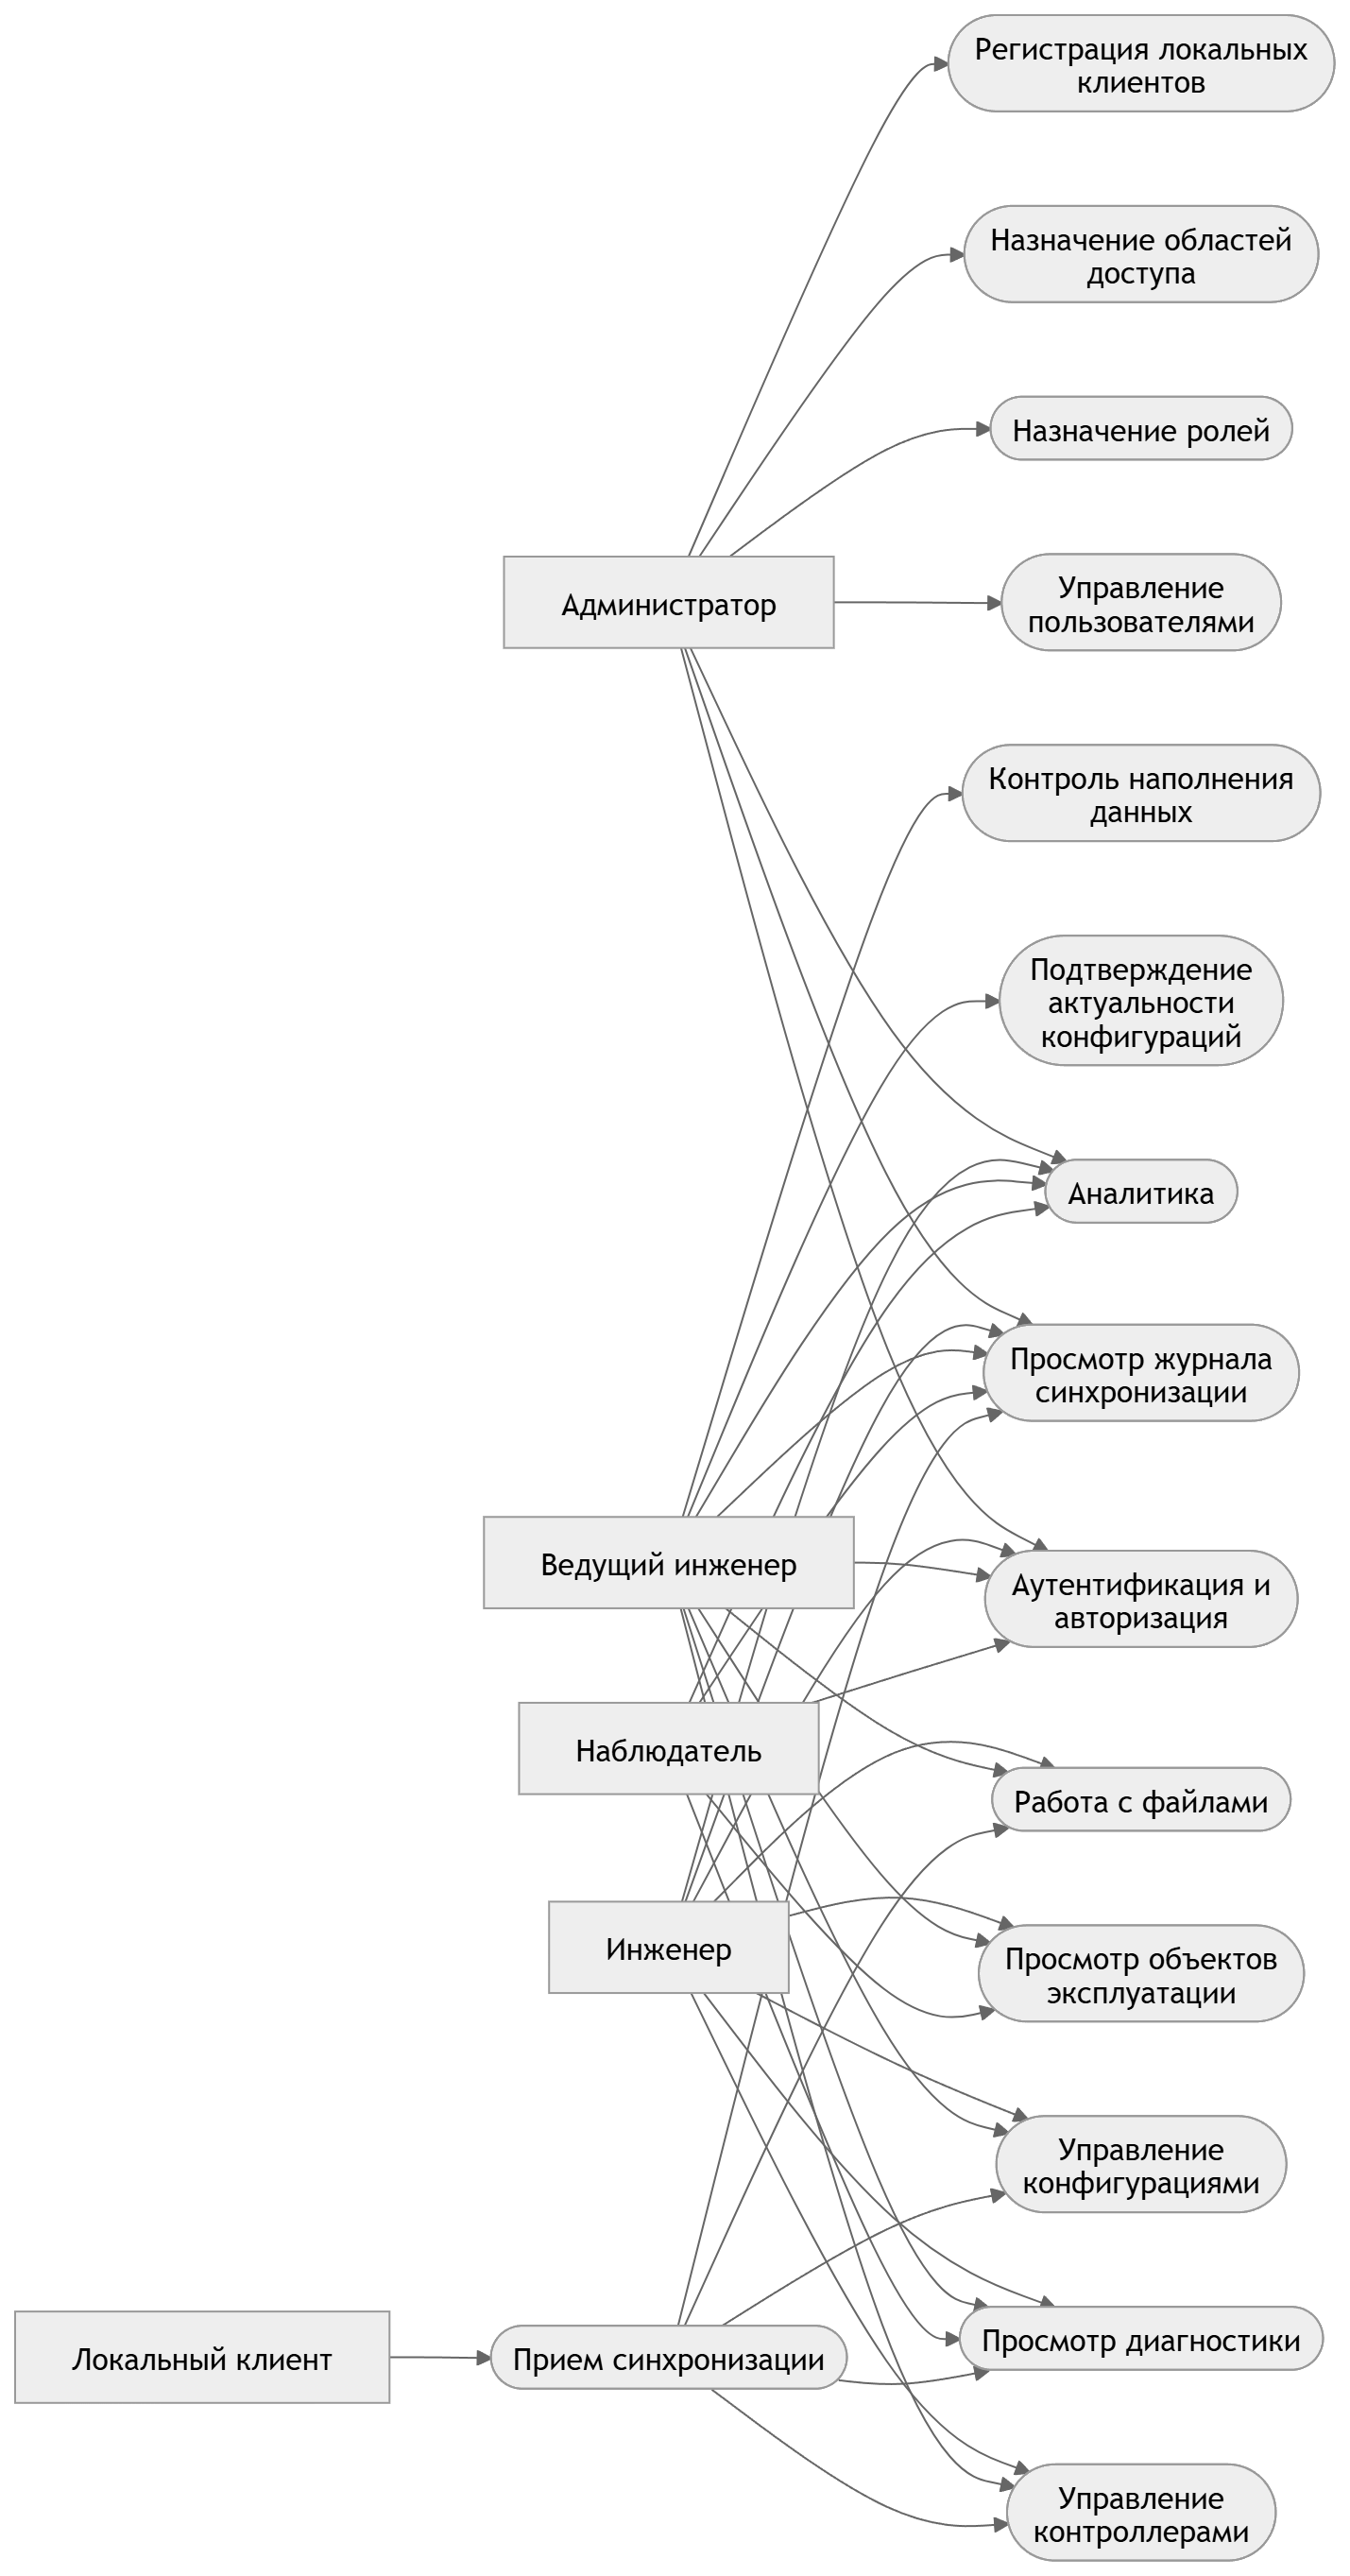
\includegraphics[width=0.90\textwidth,height=0.70\textheight,keepaspectratio]{images/diagrams/use_case.png}
	\caption{Диаграмма вариантов использования проектируемой системы}
	\label{fig:usecase2}
\end{figure}

Администратор выполняет функции настройки системы: управляет пользователями, назначает роли, назначает области доступа и регистрирует локальные клиенты. Инженер работает с эксплуатационными данными по закрепленным объектам: объектами эксплуатации, контроллерами, конфигурациями, диагностикой, файлами и результатами синхронизации. Ведущий инженер дополнительно выполняет контрольные функции: подтверждает актуальность конфигураций, проверяет полноту наполнения карточек контроллеров и анализирует состояние объектов. Наблюдатель имеет только функции просмотра. Локальный клиент участвует только в сценарии передачи данных на сервер и не получает доступа к пользовательскому интерфейсу.



\subsubsection{User story}

Для уточнения ожидаемого поведения системы были сформулированы типовые пользовательские истории:
\begin{itemize}
	\item как администратор, я хочу создавать пользователей, назначать им роли и области доступа, чтобы каждый сотрудник работал только с теми объектами, за которые он отвечает;
	\item как администратор, я хочу регистрировать локальные клиенты и привязывать их к конкретным объектам эксплуатации, чтобы данные синхронизации не попадали в систему без контроля источника;
	\item как инженер, я хочу видеть список только закрепленных за мной объектов эксплуатации, чтобы работать с нужными ПЛК без доступа к чужим промышленным данным;
	\item как инженер, я хочу вести карточки контроллеров, загружать конфигурации, журналы и файлы, чтобы фиксировать результаты сопровождения оборудования;
	\item как инженер, я хочу просматривать диагностические записи с фильтрами по объекту, ПЛК, уровню события и периоду, чтобы быстрее находить проблемы в работе оборудования;
	\item как ведущий инженер, я хочу видеть сводную аналитику по закрепленным объектам, чтобы оценивать состояние контроллеров, частоту диагностических событий и результаты синхронизаций;
	\item как ведущий инженер, я хочу подтверждать актуальность выбранной конфигурации контроллера, чтобы в системе было понятно, какая версия считается проверенной и рабочей;
	\item как ведущий инженер, я хочу контролировать полноту карточек ПЛК и наличие связанных файлов, чтобы база не превращалась в набор разрозненных записей;
	\item как наблюдатель, я хочу просматривать разрешенные объекты, диагностику, файлы и журнал синхронизации без права изменения, чтобы использовать систему для контроля и аудита;
	\item как локальный клиент, я хочу передавать на сервер результаты локального сбора данных по привязанному объекту, чтобы данные, полученные инженером на объекте без доступа к Интернету, затем попадали в общую базу.
\end{itemize}

\subsubsection{Сценарии работы пользователей}

Ключевые сценарии работы системы можно представить следующим образом.

\textbf{Сценарий 1. Настройка пользователей, ролей и областей доступа.} Администратор входит в систему, открывает раздел управления пользователями, создает или редактирует учетную запись сотрудника, назначает ему роль и указывает область доступа. Например, инженеру назначается роль инженера и объект эксплуатации ШУ ВОМ, а ведущему инженеру назначается участок вентиляции, включающий несколько шкафов. После сохранения настроек пользователь получает доступ только к тем функциям и данным, которые соответствуют его роли и области ответственности.

\textbf{Сценарий 2. Регистрация локального клиента.} Администратор открывает раздел синхронизации и регистрирует локальный клиент, который будет использоваться на ноутбуке инженера. При регистрации задаются имя клиента, ответственный пользователь и объект эксплуатации, по которому клиент имеет право передавать данные. В результате сервер формирует отдельные учетные данные для клиента. Это позволяет принимать данные синхронизации без хранения пароля пользователя в локальной программе.

\textbf{Сценарий 3. Работа инженера с контроллерами и конфигурациями.} Инженер проходит аутентификацию и видит только закрепленные за ним объекты эксплуатации. После выбора объекта он открывает список контроллеров, переходит в карточку ПЛК, проверяет основные сведения, загружает новую конфигурацию или связанный файл. Сервер проверяет право доступа к объекту, сохраняет метаданные в базе данных, а файл размещает в файловом хранилище.

\textbf{Сценарий 4. Анализ диагностических записей инженером.} Инженер открывает журнал диагностики, выбирает объект эксплуатации, контроллер, уровень события и период. Система возвращает только те диагностические записи, которые относятся к разрешенным объектам. По результатам просмотра инженер может открыть карточку контроллера, скачать связанный файл или сравнить диагностические события с историей конфигураций.

\textbf{Сценарий 5. Контроль данных ведущим инженером.} Ведущий инженер открывает панель аналитики по закрепленному участку или группе объектов. Система показывает сводные сведения о контроллерах, количестве диагностических событий, последних синхронизациях и конфигурациях, ожидающих проверки. После проверки ведущий инженер может отметить выбранную конфигурацию как актуальную, оставить комментарий и тем самым зафиксировать проверенную версию данных.

\textbf{Сценарий 6. Контроль полноты наполнения ведущим инженером.} Ведущий инженер просматривает список контроллеров, у которых отсутствуют актуальные конфигурации, вложенные файлы или свежие данные синхронизации. Такие записи требуют дополнительной проверки инженером. В результате система используется не только как хранилище, но и как инструмент контроля качества эксплуатационных данных.

\textbf{Сценарий 7. Просмотр данных наблюдателем.} Наблюдатель входит в систему и получает доступ к страницам просмотра разрешенных объектов, карточек контроллеров, диагностических записей, файлов и сессий синхронизации. При попытке выполнить изменение, загрузку файла или подтверждение конфигурации система должна отказать в выполнении операции, так как роль наблюдателя не содержит соответствующих прав.

\textbf{Сценарий 8. Прием данных от локального клиента.} Локальный клиент собирает сведения о контроллерах в локальной сети объекта и формирует пакет синхронизации. При подключении к серверу клиент передает пакет по API. Сервер проверяет подлинность клиента и его привязку к объекту эксплуатации, создает запись сессии синхронизации, сохраняет контроллеры, конфигурации, диагностические записи и файлы. После обработки данные становятся доступны инженеру и ведущему инженеру в пределах их областей доступа.

Перечисленные сценарии показывают, что система не ограничивается простой загрузкой файлов. Она связывает роли пользователей, области доступа, карточки контроллеров, конфигурации, диагностику, файлы и сессии синхронизации в единую модель сопровождения ПЛК LogicBox.

\subsection{Проектирование модели данных}

Проектирование модели данных необходимо для определения состава сущностей системы, их атрибутов и взаимосвязей. Веб-приложение должно поддерживать хранение справочной информации о контроллерах, историю конфигураций, диагностические записи, файловые вложения, области доступа и сессии синхронизации.

\subsubsection{Состав сущностей предметной модели}

В модели данных веб-приложения выделяются сущности, необходимые для учета пользователей, объектов эксплуатации, контроллеров LogicBox, конфигураций, диагностических записей, файловых вложений, сессий синхронизации и событий аудита. Их взаимосвязи представлены на \figref{fig:erdconcept2}.

\begin{figure}[H]
    \centering
    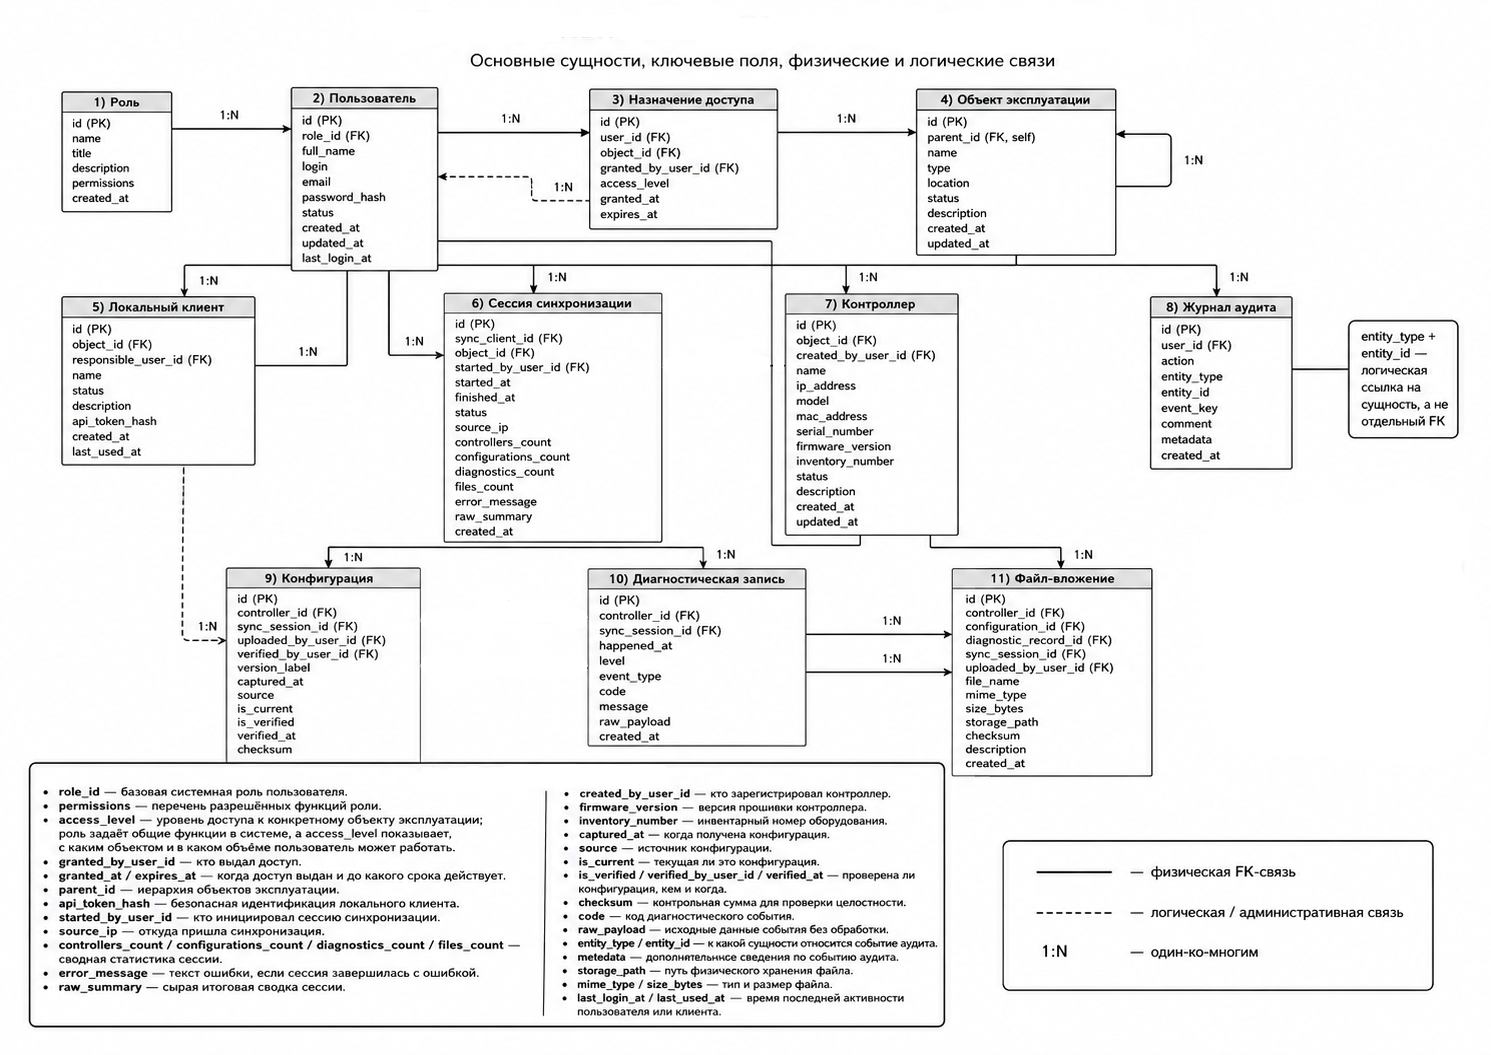
\includegraphics[width=0.90\textwidth,height=0.70\textheight,keepaspectratio]{images/diagrams/erd_concept.png}
    \caption{Концептуальная ER-диаграмма предметной области}
    \label{fig:erdconcept2}
\end{figure}

Центральной сущностью модели является объект эксплуатации. Под объектом эксплуатации понимается площадка, шкаф управления, стенд, участок АСУТП или иной логический контур, в пределах которого размещаются контроллеры LogicBox и ведется инженерная работа. Объекты эксплуатации могут образовывать иерархию за счет поля \texttt{parent\_id}: например, предприятие может включать несколько участков, а участок --- несколько шкафов управления. Такая структура позволяет назначать доступ не только к отдельному объекту, но и к группе связанных объектов.

Сущность \texttt{users} хранит учетные записи пользователей системы. Сущность \texttt{roles} задает базовую системную роль пользователя: администратор, инженер, ведущий инженер, наблюдатель и другие роли, предусмотренные системой. Роль определяет, какие функции пользователь в принципе может выполнять в веб-приложении: просматривать данные, создавать записи, загружать файлы, подтверждать конфигурации, управлять пользователями или назначать области доступа.

Отдельно от роли используется сущность \texttt{user\_object\_access}, предназначенная для назначения пользователю доступа к конкретным объектам эксплуатации. Это разделение необходимо потому, что роль и область доступа решают разные задачи. Роль отвечает на вопрос, какие действия пользователь может выполнять в системе в целом, а назначение доступа отвечает на вопрос, с какими именно объектами эксплуатации пользователь может работать. Например, два пользователя могут иметь одинаковую роль инженера, но один из них должен работать только с объектом ШУ ВОМ, а другой --- только со стендом LogicBox или отдельным участком АСУТП.

Поле \texttt{access\_level} в таблице назначений доступа используется для уточнения уровня доступа пользователя к конкретному объекту эксплуатации. Наличие этого поля не дублирует роль, а дополняет ее. Роль задает общий набор разрешенных функций, а \texttt{access\_level} ограничивает или расширяет эти функции в рамках конкретного объекта. Например, пользователь с инженерной ролью может иметь полный доступ к одному объекту, доступ только на просмотр к другому объекту и не иметь доступа к остальным объектам. Без такого поля пришлось бы создавать большое количество отдельных ролей под каждую комбинацию объекта и прав, что сделало бы модель доступа неудобной и плохо масштабируемой.

Сущность \texttt{sync\_clients} описывает локальные клиенты синхронизации. Локальный клиент не является пользователем веб-интерфейса. Это внешний программный компонент, который работает на объекте эксплуатации, собирает данные о контроллерах в локальной сети и передает их на сервер через API. Для безопасной идентификации клиента используется поле \texttt{api\_token\_hash}, в котором хранится не сам токен, а его хэш. Это снижает риск компрометации доступа при утечке данных из базы.

Сущность \texttt{sync\_sessions} фиксирует отдельные сессии синхронизации. Каждая сессия связана с локальным клиентом, объектом эксплуатации и пользователем, который инициировал синхронизацию, если такая операция была выполнена из пользовательского сценария. В сессии сохраняются время начала и завершения, статус обработки, IP-адрес источника, количество обработанных контроллеров, конфигураций, диагностических записей и файлов. Поля \texttt{error\_message} и \texttt{raw\_summary} позволяют хранить сведения об ошибках и исходную итоговую сводку синхронизации. Благодаря этому можно проследить, когда и откуда данные попали в систему.

Сущность \texttt{controllers} хранит карточки контроллеров LogicBox. Контроллер привязывается к объекту эксплуатации и содержит эксплуатационные сведения: имя, IP-адрес, модель, MAC-адрес, серийный номер, версию прошивки, инвентарный номер, статус и описание. Через поле \texttt{created\_by\_user\_id} фиксируется пользователь, зарегистрировавший контроллер в системе. Контроллер является основной инженерной сущностью, вокруг которой группируются конфигурации, диагностические записи и файлы.

Сущность \texttt{configurations} используется для хранения истории конфигураций контроллеров. Каждая конфигурация связана с контроллером и при необходимости с сессией синхронизации, в рамках которой она была получена. Поля \texttt{version\_label}, \texttt{captured\_at} и \texttt{source} позволяют определить версию, время получения и источник конфигурации. Поле \texttt{is\_current} показывает, является ли конфигурация текущей для контроллера, а поля \texttt{is\_verified}, \texttt{verified\_by\_user\_id} и \texttt{verified\_at} фиксируют факт проверки конфигурации ответственным специалистом. Поле \texttt{checksum} используется для контроля целостности данных.

Сущность \texttt{diagnostic\_records} предназначена для хранения диагностических событий контроллеров. Диагностическая запись связана с контроллером и может быть связана с сессией синхронизации. В ней фиксируются время события, уровень важности, тип события, код, текст сообщения и исходные данные события в поле \texttt{raw\_payload}. Такое разделение позволяет хранить как обработанное описание события, удобное для просмотра пользователем, так и исходные данные, полученные от локального клиента.

Сущность \texttt{attachments} хранит метаданные файловых вложений. Файл может быть связан с контроллером, конфигурацией, диагностической записью или сессией синхронизации. В базе данных сохраняются имя файла, тип \texttt{mime\_type}, размер \texttt{size\_bytes}, путь физического хранения \texttt{storage\_path}, контрольная сумма и описание. Само бинарное содержимое файла хранится во внешнем файловом хранилище. Такой подход позволяет не перегружать основную базу данных крупными файлами и упрощает резервное копирование.

Сущность \texttt{audit\_events} используется для ведения журнала аудита. Каждое событие аудита связано с пользователем через поле \texttt{user\_id}. Поля \texttt{action}, \texttt{event\_key}, \texttt{comment} и \texttt{metadata} позволяют зафиксировать действие пользователя, служебный код события, пояснение и дополнительные сведения. Поля \texttt{entity\_type} и \texttt{entity\_id} образуют логическую ссылку на сущность, к которой относится событие аудита. Это не отдельный внешний ключ на объект эксплуатации, а универсальный механизм ссылки на разные типы сущностей: пользователя, контроллер, конфигурацию, файл, сессию синхронизации и другие записи. Поэтому на концептуальной диаграмме эта связь выделяется как логическая.

Таким образом, предметная модель отражает не только хранение данных о ПЛК LogicBox, но и эксплуатационную логику системы: пользователь получает доступ к конкретным объектам, объект объединяет контроллеры, контроллер имеет историю конфигураций и диагностики, а происхождение данных прослеживается через сессии синхронизации и журнал аудита.

\subsubsection{Логическая схема данных}

На логическом уровне каждая сущность предметной области представляется отдельной таблицей. Между таблицами используются связи типа <<один-ко-многим>>, поскольку один объект эксплуатации может содержать несколько контроллеров, один контроллер может иметь несколько конфигураций, диагностических записей и файлов, а один пользователь может быть связан с несколькими действиями, назначениями доступа и загруженными материалами.

Связь между таблицами \texttt{roles} и \texttt{users} отражает принадлежность пользователя к базовой роли. Эта связь используется для определения общего набора функций, доступных пользователю в системе. При этом роль не определяет конкретные промышленные объекты, с которыми работает пользователь.

Связь между \texttt{users}, \texttt{exploitation\_objects} и \texttt{user\_object\_access} реализует модель разграничения доступа по объектам эксплуатации. Таблица \texttt{user\_object\_access} является связующей таблицей между пользователями и объектами. Она позволяет назначить одному пользователю доступ к нескольким объектам, а к одному объекту --- доступ нескольким пользователям. Поле \texttt{access\_level} уточняет уровень доступа в рамках конкретного объекта, например просмотр, редактирование или расширенные инженерные действия. За счет этого система поддерживает одновременно ролевое разграничение и разграничение по зоне ответственности.

Связь \texttt{exploitation\_objects.parent\_id} с \texttt{exploitation\_objects.id} используется для построения иерархии объектов эксплуатации. Такая связь позволяет описывать вложенные структуры: предприятие, участок, шкаф управления, стенд или отдельный контур автоматизации. Это важно для инженерной системы, поскольку контроллеры редко существуют изолированно и обычно относятся к конкретному объекту или группе объектов.

Таблица \texttt{sync\_clients} связана с объектами эксплуатации и пользователями. Объект эксплуатации определяет, по какому объекту локальный клиент имеет право передавать данные, а ответственный пользователь позволяет понять, кто отвечает за работу данного клиента. При выполнении обмена создается запись в таблице \texttt{sync\_sessions}. Каждая сессия синхронизации связана с локальным клиентом, объектом эксплуатации и пользователем-инициатором. Это позволяет отделить постоянную регистрацию клиента от конкретных фактов обмена данными.

Таблица \texttt{controllers} связана с объектом эксплуатации, поскольку каждый контроллер должен относиться к конкретному объекту или участку. Дополнительно фиксируется пользователь, зарегистрировавший контроллер. От контроллера зависят конфигурации, диагностические записи и файловые вложения. Такая структура отражает реальную эксплуатационную логику: контроллер является устройством, по которому накапливаются версии конфигураций, события диагностики и сопроводительные файлы.

Таблица \texttt{configurations} связана с контроллером и сессией синхронизации. Связь с контроллером показывает, к какому ПЛК относится конфигурация, а связь с сессией синхронизации показывает, в рамках какого обмена данные были получены. Также конфигурация связана с пользователями: один пользователь мог загрузить конфигурацию, другой --- проверить и подтвердить ее. На концептуальной диаграмме такие административные связи могут быть выделены отдельно, поскольку они отражают не принадлежность данных, а ответственность за действие.

Таблица \texttt{diagnostic\_records} связана с контроллером и сессией синхронизации. Это позволяет просматривать диагностические события как в карточке конкретного ПЛК, так и в контексте конкретного импорта данных от локального клиента. Такая связь полезна при анализе повторяющихся ошибок и при проверке того, какие события были получены во время конкретной синхронизации.

Таблица \texttt{attachments} связана сразу с несколькими инженерными сущностями: контроллером, конфигурацией, диагностической записью и сессией синхронизации. Это сделано для того, чтобы один механизм файловых вложений можно было использовать в разных разделах системы. Например, файл может быть общей документацией по контроллеру, файлом конфигурации, приложением к диагностическому событию или материалом, полученным в рамках синхронизации. При этом автор загрузки фиксируется через связь с пользователем.

Таблица \texttt{audit\_events} связана с пользователем физическим внешним ключом \texttt{user\_id}. Остальная привязка события аудита выполняется через поля \texttt{entity\_type} и \texttt{entity\_id}. Это универсальная логическая ссылка, позволяющая записывать события по разным сущностям без создания отдельного внешнего ключа для каждого возможного типа записи. Такой подход делает журнал аудита расширяемым и не привязывает его только к объектам эксплуатации или контроллерам.

Следовательно, логическая схема данных поддерживает полный цикл работы системы: настройку пользователей и ролей, назначение областей доступа, регистрацию объектов и контроллеров, прием данных от локального клиента, хранение конфигураций и диагностики, работу с файлами и аудит действий пользователей.

\subsubsection{Физическая схема базы данных}

Для реализации хранилища данных используется реляционная СУБД PostgreSQL \cite{postgresql_official}. PostgreSQL поддерживает внешние ключи, транзакции, индексацию, типы данных для времени, сетевых адресов и JSON-структур, что соответствует задачам проектируемого веб-приложения. Физическая ERD-схема базы данных представлена на \figref{fig:erdphysical2}.

\begin{figure}[H]
    \centering
    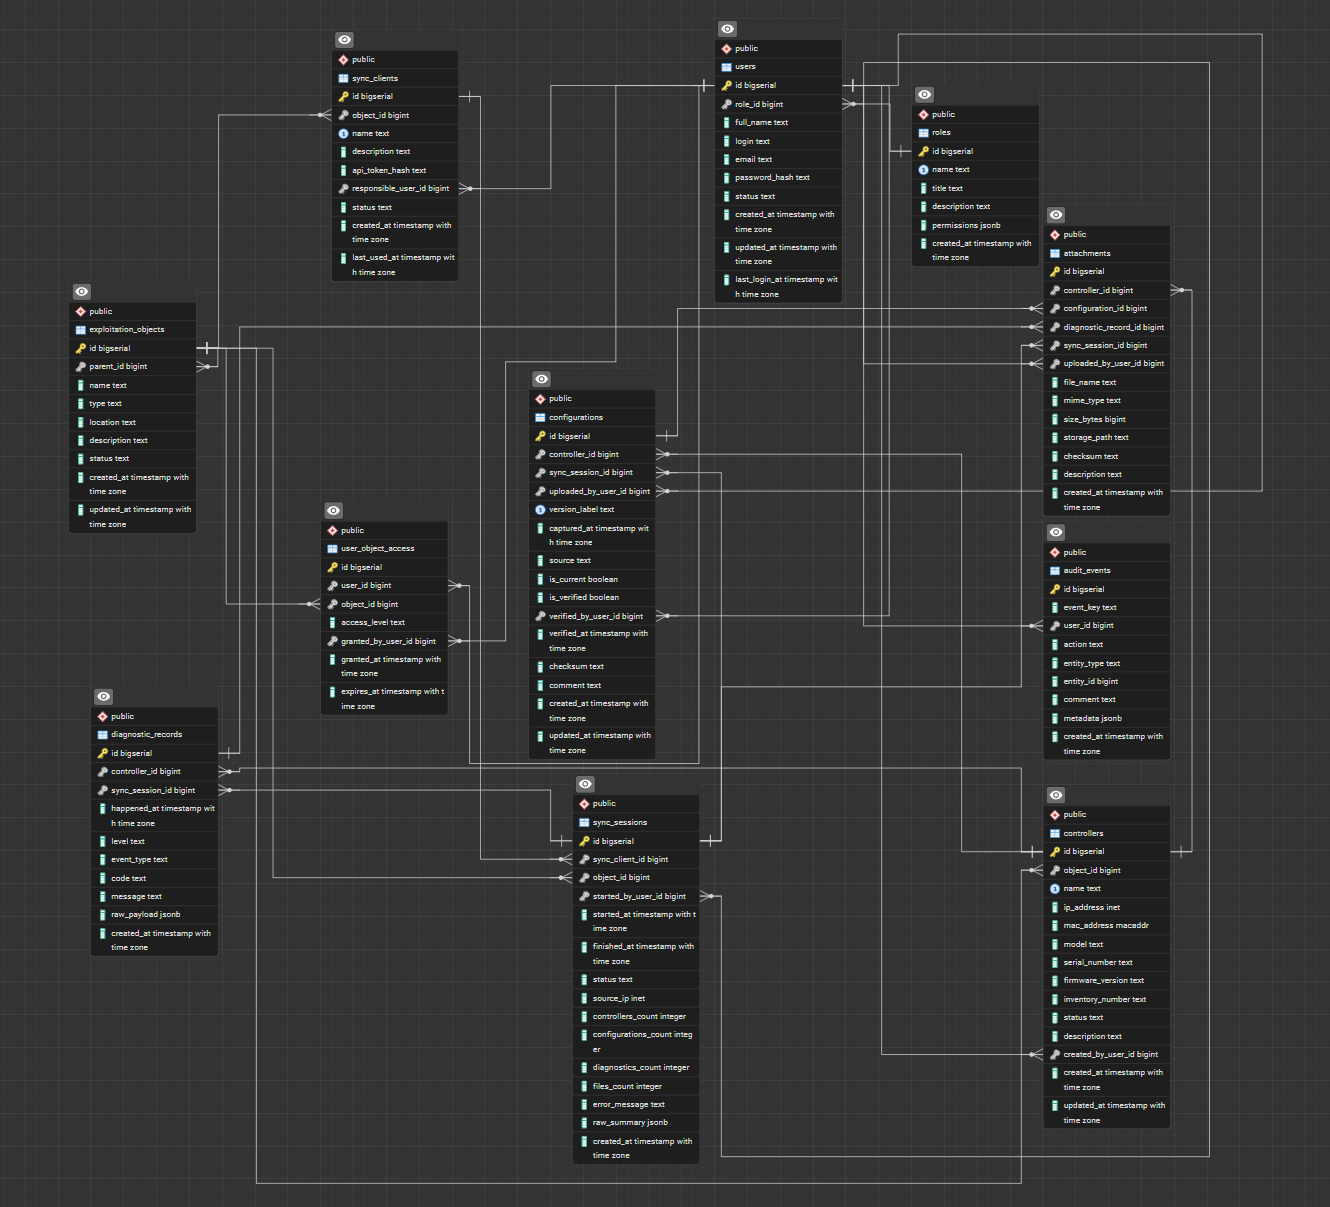
\includegraphics[width=0.90\textwidth,height=0.70\textheight,keepaspectratio]{images/diagrams/erd_physical.png}
    \caption{Физическая ERD-схема базы данных}
    \label{fig:erdphysical2}
\end{figure}

Физическая схема уточняет логическую модель и показывает реальные таблицы, поля, типы данных и связи по внешним ключам. Первичные ключи таблиц реализуются полями \texttt{id} типа \texttt{bigserial}. Внешние ключи используют поля типа \texttt{bigint}, ссылающиеся на идентификаторы связанных записей. Текстовые сведения, такие как наименования, статусы, комментарии, версии и сообщения диагностики, хранятся в полях типа \texttt{text}. Даты и время фиксируются с помощью типа \texttt{timestamp with time zone}, что позволяет корректно учитывать время создания, обновления, синхронизации и проверки записей.

Для хранения дополнительных структурированных данных используются поля типа \texttt{jsonb}. В частности, \texttt{permissions} в таблице ролей может хранить набор разрешений роли, \texttt{raw\_summary} в сессии синхронизации --- исходную сводку обработки, \texttt{raw\_payload} в диагностической записи --- исходные данные события, а \texttt{metadata} в журнале аудита --- дополнительные сведения о действии пользователя. Использование \texttt{jsonb} позволяет хранить расширяемые данные без постоянного изменения структуры таблиц при добавлении новых служебных параметров.

В таблице \texttt{controllers} поле \texttt{ip\_address} хранит сетевой адрес контроллера, а поле \texttt{mac\_address} хранит MAC-адрес устройства. Эти поля используются для идентификации оборудования в локальной сети и сопоставления данных, полученных от локального клиента. Поля \texttt{serial\_number}, \texttt{firmware\_version} и \texttt{inventory\_number} позволяют вести эксплуатационный учет оборудования.

Физическая схема сохраняет принцип разделения роли и объектного доступа. Таблица \texttt{users} содержит поле \texttt{role\_id}, определяющее системную роль пользователя. Таблица \texttt{user\_object\_access} содержит поля \texttt{user\_id}, \texttt{object\_id} и \texttt{access\_level}, определяющие доступ пользователя к конкретному объекту эксплуатации. Поэтому при проверке прав сервер должен учитывать два условия: разрешает ли роль выполнить действие и есть ли у пользователя доступ к объекту, с которым связаны запрашиваемые данные.

Схема также обеспечивает прослеживаемость происхождения данных. Если конфигурация, диагностическая запись или файл были получены в рамках синхронизации, они связываются с записью \texttt{sync\_sessions}. Сама сессия связана с локальным клиентом и объектом эксплуатации. Благодаря этому можно определить, каким клиентом, с какого объекта, в какое время и с каким результатом данные были переданы на сервер.

Файловые вложения в физической схеме представлены таблицей \texttt{attachments}. В базе данных хранятся только метаданные файла: имя, тип, размер, путь хранения, контрольная сумма, описание, автор загрузки и связи с другими сущностями. Бинарное содержимое файла хранится отдельно в файловом хранилище. Такой подход уменьшает нагрузку на базу данных, упрощает резервное копирование и позволяет проверять целостность файла по контрольной сумме.

Журнал аудита реализован таблицей \texttt{audit\_events}. Физический внешний ключ в этой таблице указывает на пользователя, выполнившего действие. Поля \texttt{entity\_type} и \texttt{entity\_id} используются как логическая ссылка на запись, к которой относится событие. Это решение позволяет фиксировать действия по разным сущностям без усложнения схемы множеством необязательных внешних ключей.

Таким образом, физическая схема базы данных соответствует предметной модели веб-приложения и обеспечивает хранение пользователей, ролей, областей доступа, объектов эксплуатации, контроллеров, конфигураций, диагностических записей, файловых вложений, сессий синхронизации и событий аудита. При этом схема не содержит сущностей для удаленного управления ПЛК, что соответствует принятому ограничению: приложение предназначено для учета, хранения, анализа, синхронизации и аудита данных, а не для непосредственного воздействия на промышленное оборудование.

\subsection{Проектирование архитектуры интерфейсов и взаимодействия компонентов}

\subsubsection{Обоснование выбора технологического стека}

Для серверной части системы выбран стек \textbf{Go + Fiber + PostgreSQL}. Язык Go \cite{golang_official} применяется для разработки сетевых и серверных приложений, отличается статической типизацией, предсказуемой моделью развертывания и удобством сопровождения. Для системы, в которой предполагается работа с аутентификацией, ролями, файлами, фильтрацией и приемом данных от внешнего клиента, это является существенным преимуществом.

В качестве веб-фреймворка выбран Fiber \cite{fiber_official}. Он обеспечивает маршрутизацию, middleware, работу с формами, обработку JSON и статических файлов, что достаточно для построения проектируемого веб-приложения.

В учебной практике часто используется связка Python + Flask \cite{flask_official}. Она также подходит для решения задач рассматриваемого класса. Однако выбор Go + Fiber для данного проекта является рациональным по следующим причинам:
\begin{itemize}
    \item наличие практической компетенции по данному стеку снижает риск срыва сроков и повышает вероятность доведения системы до рабочего результата;
    \item Go позволяет собрать серверное приложение в единый исполняемый файл, что упрощает развертывание и переносимость;
    \item выбранный стек хорошо подходит для реализации API, работы с файлами и многопользовательских сценариев;
    \item использование Go на сервере не ограничивает архитектуру только этим языком, поскольку взаимодействие компонентов строится через HTTP-маршруты, шаблоны интерфейса и реляционную схему данных.
\end{itemize}

Таким образом, выбор Go + Fiber не означает непригодность Python + Flask, но является более рациональным для данного проекта с учетом эксплуатационной модели приложения, имеющихся компетенций и сроков выполнения курсовой работы.

\subsubsection{Обоснование выбора HTML, CSS и JavaScript для клиентской части}

Для клиентской части системы выбрана базовая связка \textbf{HTML + CSS + JavaScript} \cite{mdn_html,mdn_css,mdn_js}. Такой выбор обусловлен характером интерфейса: система преимущественно состоит из форм, таблиц, карточек сущностей, журналов и фильтров. Для подобного класса приложений не требуется тяжелая одно-страничная архитектура, если основной функционал можно реализовать с помощью серверного рендеринга шаблонов и ограниченного количества клиентских сценариев.

Дополнительным аргументом является то, что HTML-макеты, подготовленные на этапе проектирования, могут без существенной переработки быть использованы при последующей реализации системы в третьем разделе. Это позволяет избежать дублирования работы, когда сначала разрабатываются условные изображения экранов, а затем те же страницы создаются заново в коде.

\subsubsection{Архитектурная независимость от конкретного backend-стека}

Несмотря на выбор Go + Fiber в качестве основного стека реализации, архитектура приложения должна оставаться относительно независимой от конкретного фреймворка. Для этого проект закладывается как слоистая архитектура, включающая следующие уровни:
\begin{itemize}
    \item уровень представления --- HTML-страницы, формы, таблицы и клиентские сценарии;
    \item прикладной уровень --- сервисы, реализующие бизнес-логику, аутентификацию, проверку прав, работу с синхронизацией и файлами;
    \item уровень доступа к данным --- работа с базой данных и файловым хранилищем.
\end{itemize}

Подобный подход позволяет при необходимости заменить реализацию прикладного уровня с Go + Fiber на другой стек, например Python + Flask, без полного пересмотра предметной модели, маршрутов, интерфейсов и структуры базы данных.

\subsubsection{Логическая архитектура веб-приложения}

Логическая архитектура системы приведена на \figref{fig:arch2}. Диаграмма показывает, что веб-приложение взаимодействует как с пользовательским веб-интерфейсом, так и с локальным клиентом, однако все критические операции проходят через серверный слой.

\begin{figure}[H]
    \centering
    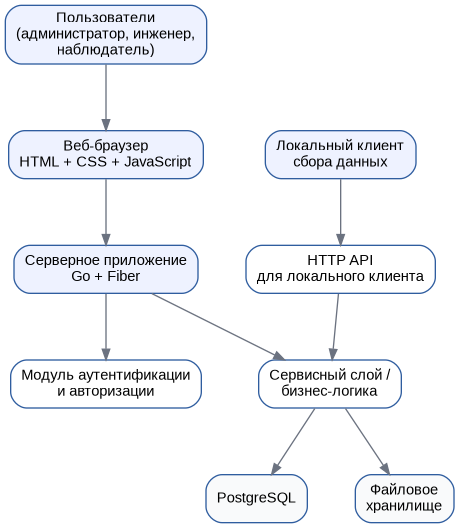
\includegraphics[width=0.90\textwidth,height=0.70\textheight,keepaspectratio]{images/diagrams/architecture.png}
    \caption{Логическая архитектура веб-приложения}
    \label{fig:arch2}
\end{figure}

Серверная часть включает модуль аутентификации и авторизации, модуль работы с пользователями и ролями, модуль учета объектов эксплуатации и контроллеров, модуль конфигураций, модуль диагностики, модуль вложений и модуль синхронизации. Все модули используют общую базу данных и файловое хранилище.

\subsubsection{Архитектура загрузки и выгрузки файлов}

Файлы в системе используются для хранения конфигураций, журналов, отчетов и вспомогательных материалов. При загрузке файла пользователь или внешний клиент передает файл на сервер. Сервер выполняет валидацию типа и размера файла, вычисляет метаданные и сохраняет бинарное содержимое в отдельном файловом хранилище. В базе данных при этом фиксируются имя файла, тип, размер, путь хранения, контрольная сумма, автор загрузки и связь с соответствующей сущностью.

При выгрузке файл извлекается по ссылке из карточки сущности, при этом сервер дополнительно проверяет право пользователя на доступ к связанной записи. Такой подход позволяет реализовать обязательное требование курсового проекта по загрузке и выгрузке файлов без смешивания файлового и табличного хранения.

\subsubsection{Взаимодействие сервера с локальным клиентом}

Последовательность взаимодействия сервера с локальным клиентом приведена на \figref{fig:syncsequence2}.

\begin{figure}[H]
    \centering
    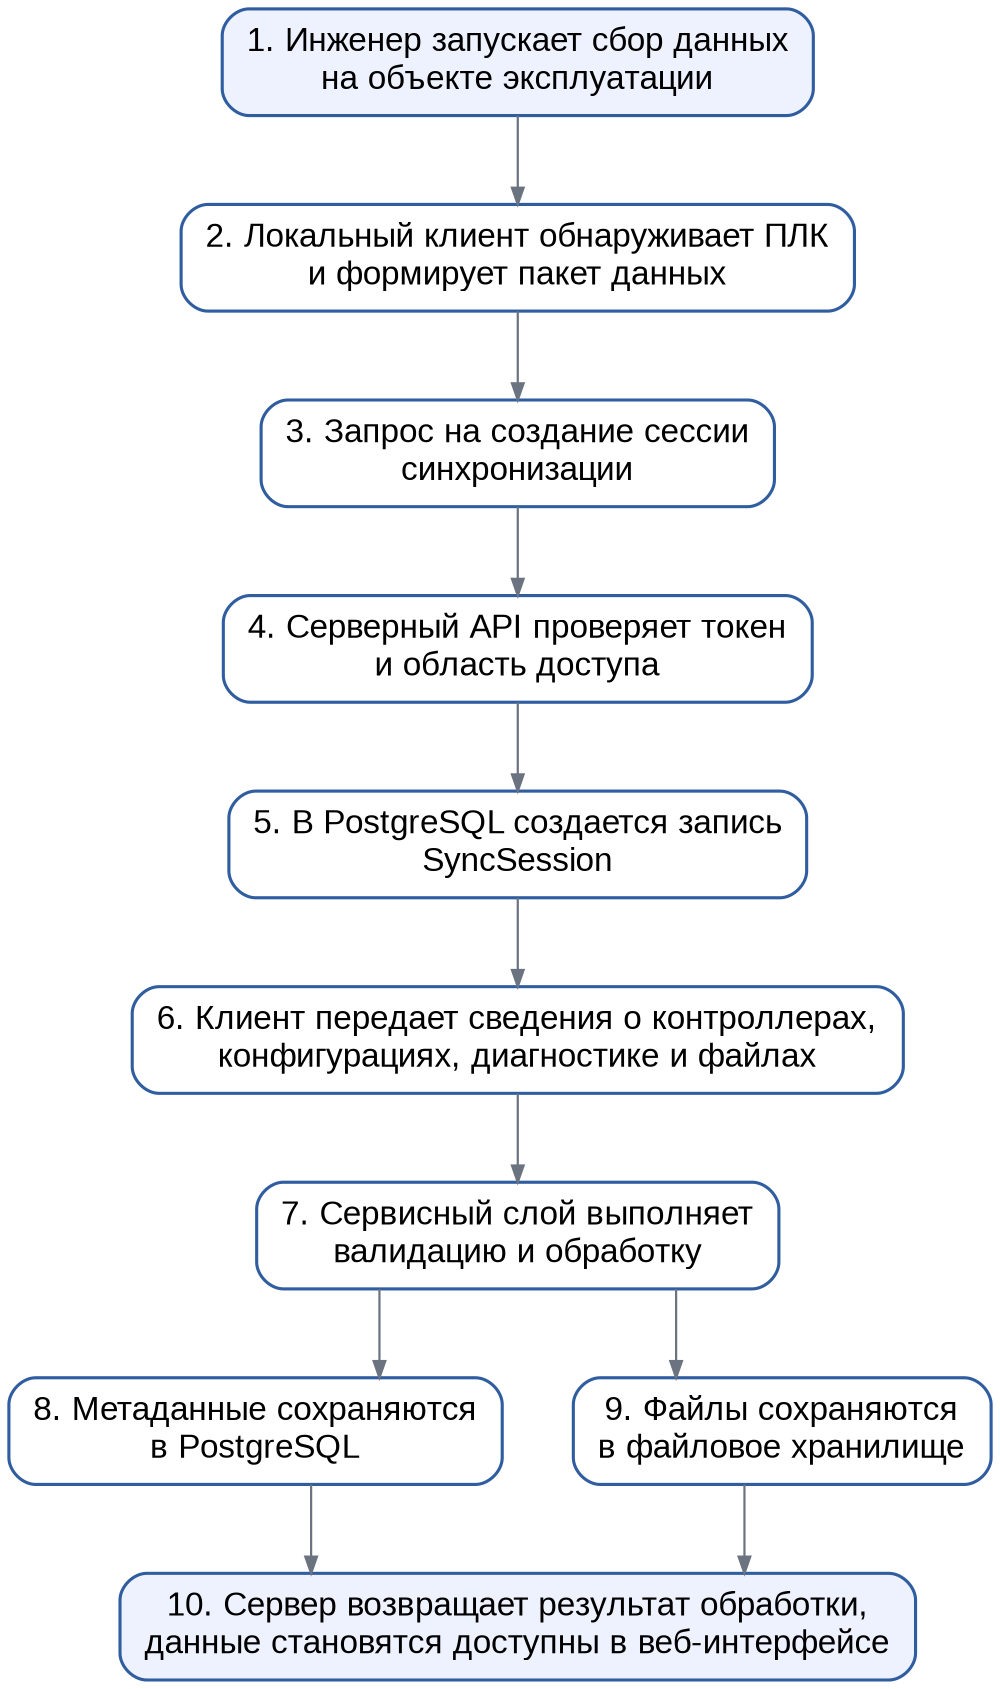
\includegraphics[width=0.90\textwidth,height=0.70\textheight,keepaspectratio]{images/diagrams/sync_sequence.png}
    \caption{Последовательность взаимодействия локального клиента и сервера}
    \label{fig:syncsequence2}
\end{figure}

Локальный клиент собирает данные в локальной сети объекта, формирует пакет и передает его на сервер по защищенному API. Сервер аутентифицирует клиента, создает запись сессии синхронизации, сохраняет переданные сведения и возвращает результат обработки. Далее импортированные данные становятся доступны в веб-интерфейсе пользователям с соответствующими правами.

\subsubsection{Макеты пользовательского интерфейса}

Для проектируемого приложения подготовлены HTML-макеты основных пользовательских страниц и модальных окон. Чтобы не перегружать основной текст большим количеством иллюстраций, макеты вынесены в \hyperref[sec:appendix_mockups]{приложение~А}. В основном тексте приведено описание их назначения и связи с функциями системы.

Страница входа предназначена для аутентификации пользователя и проверки его учетных данных. Помимо логина и пароля, в макете предусмотрено поле для кода подтверждения при включенной двухфакторной аутентификации. Данное поле используется только для тех учетных записей, у которых включена дополнительная проверка входа: после ввода логина и пароля пользователь указывает одноразовый код из приложения-аутентификатора. Если двухфакторная аутентификация для пользователя не включена, поле не участвует в проверке входа.

После успешного входа сервер определяет роль пользователя и список разрешенных объектов эксплуатации. Панели инженера, администратора и наблюдателя отражают различия в доступных функциях: инженер работает с объектами, контроллерами, конфигурациями, диагностикой и синхронизацией; администратор управляет учетными записями, ролями и областями доступа; наблюдатель получает только режим просмотра.

Макеты реестра объектов эксплуатации и карточки объекта связаны с таблицами объектов эксплуатации и назначений доступа пользователей. Через эти страницы пользователь видит только те площадки, шкафы или стенды, которые находятся в его области ответственности. Макеты списка контроллеров и карточки контроллера связаны с таблицей контроллеров; через карточку контроллера открываются связанные конфигурации, диагностические записи, вложения и сессии синхронизации.

Макеты страниц конфигураций, диагностики, файлов-вложений и сессий синхронизации отражают работу с таблицами конфигураций, диагностических записей, файловых вложений и сессий синхронизации. Модальные окна используются для операций создания и редактирования сущностей, загрузки конфигураций и файлов, регистрации локального клиента и назначения областей доступа. Такой подход позволяет не перегружать основные страницы большим количеством форм и оставить структуру интерфейса понятной для пользователей разных ролей.

